

\begin{figure}[t]
\centering
 
\includegraphics[width=6in]{submissions/Jing2024/figures/experiments/relation_analysis/legend.pdf}
\\\vspace{-6mm}
\subfloat[\textit{Correctness} vs Head entity type]{
 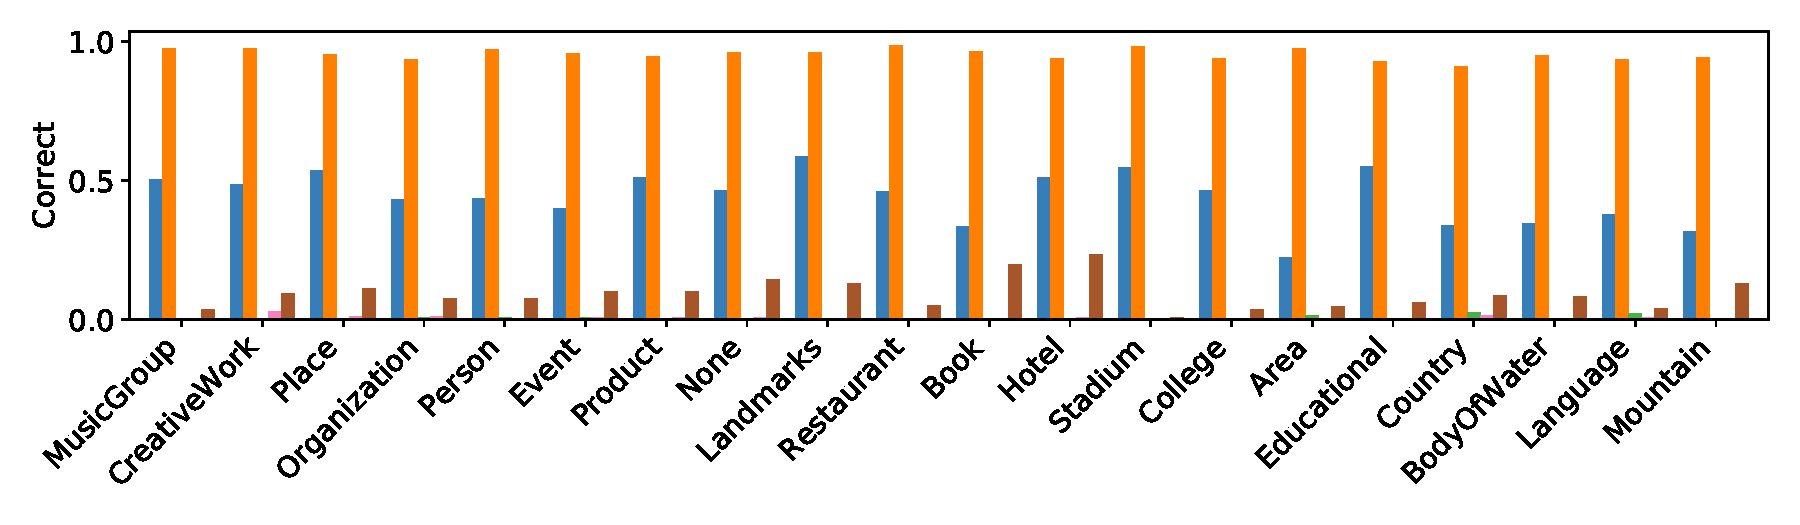
\includegraphics[width=5.5in]{submissions/Jing2024/figures/experiments/relation_analysis/correct_by_head_type.pdf}
 \label{fig:correct_by_head_type}
}\\

\includegraphics[width=5.5in]{submissions/Jing2024/figures/experiments/relation_analysis/legend.pdf}
\\\vspace{-6mm}
\subfloat[\textit{Correctness} vs Tail entity type]{
 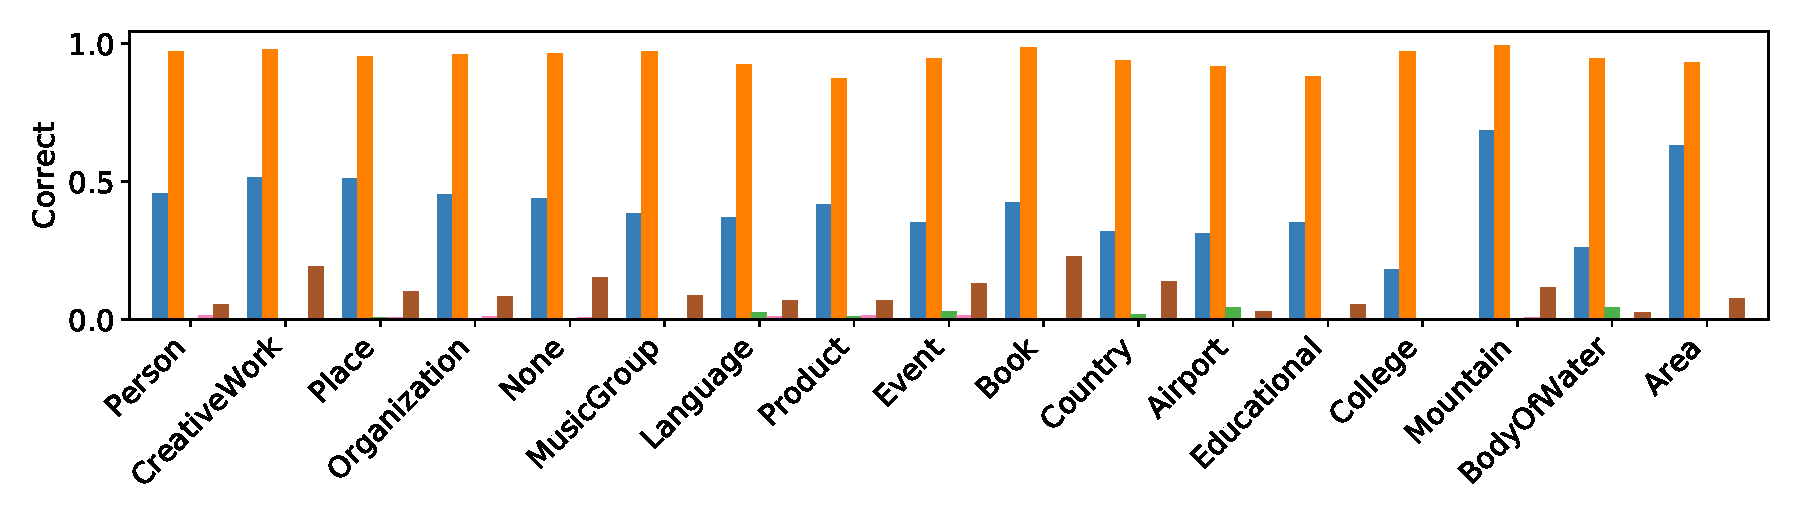
\includegraphics[width=5.5in]{submissions/Jing2024/figures/experiments/relation_analysis/correct_by_tail_type.pdf}
 \label{fig:correct_by_tail_type}
}
\caption{The LLM's \textit{correctness} with respect to head entity types and tail entity types}
\label{fig:correctness_by_type}
\end{figure}


\begin{figure}[t]
    \centering
 
\includegraphics[width=5.5in]{submissions/Jing2024/figures/experiments/relation_analysis/legend.pdf}
 \\\vspace{-6mm}
\subfloat[\textit{Truthfulness} vs Head entity type]{
 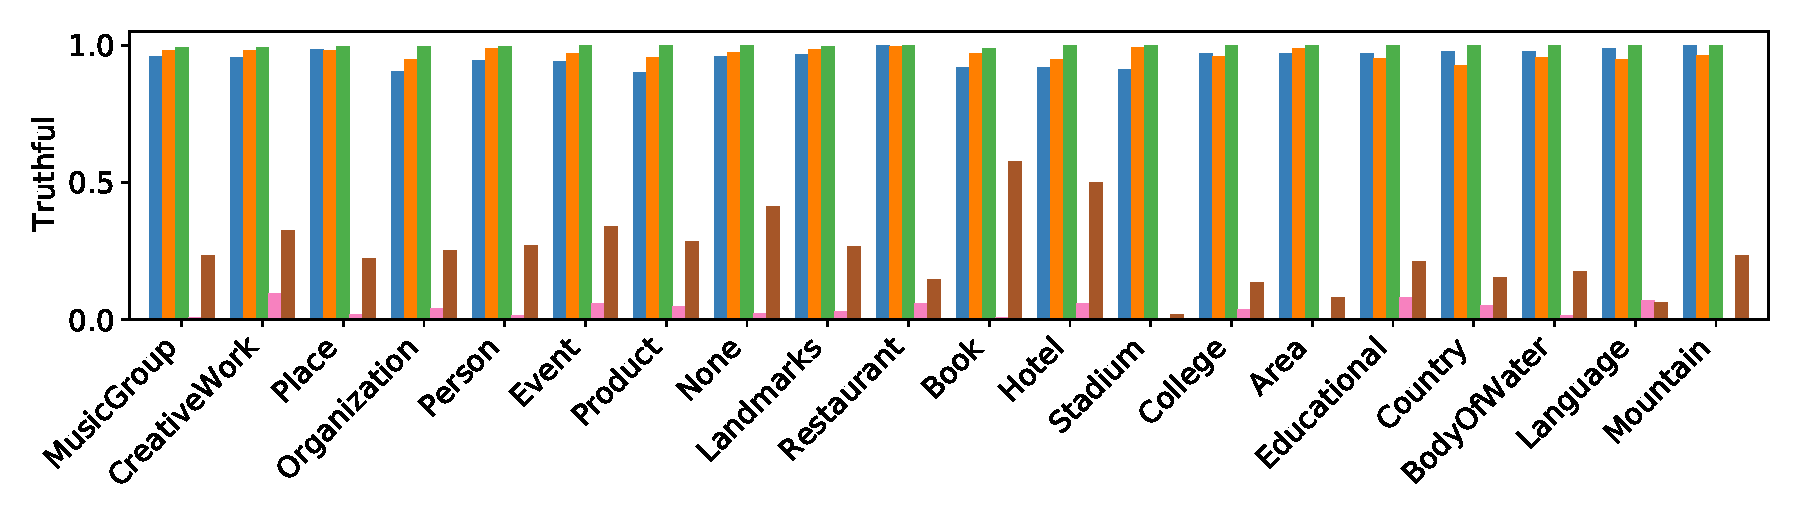
\includegraphics[width=5.5in]{submissions/Jing2024/figures/experiments/relation_analysis/truthful_by_head_type.pdf}
 \label{fig:truthful_by_head_type}
}\\

\includegraphics[width=5.5in]{submissions/Jing2024/figures/experiments/relation_analysis/legend.pdf}
\\\vspace{-6mm}
\subfloat[\textit{Truthfulness} vs Tail entity type]{
 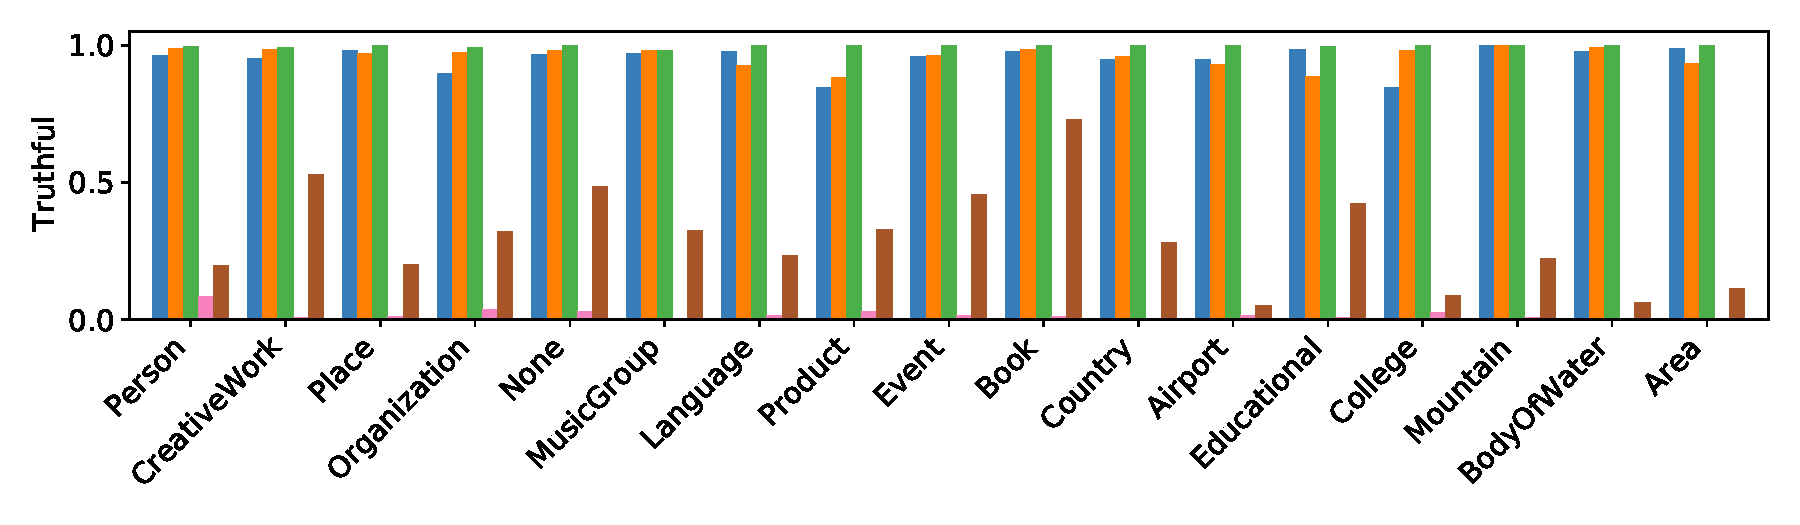
\includegraphics[width=5.5in]{submissions/Jing2024/figures/experiments/relation_analysis/truthful_by_tail_type.pdf}
 \label{fig:truthful_by_tail_type}
}
\caption{The LLM's \textit{truthfulness} with respect to head entity types and tail entity types}
\label{fig:truthfulness_by_type}
\end{figure}
\begin{figure}[t]
    \centering
    
\includegraphics[width=6in]{submissions/Jing2024/figures/experiments/relation_analysis/legend.pdf}
    \\\vspace{-6mm}
\subfloat[\textit{Informativeness} vs Head entity type]{
 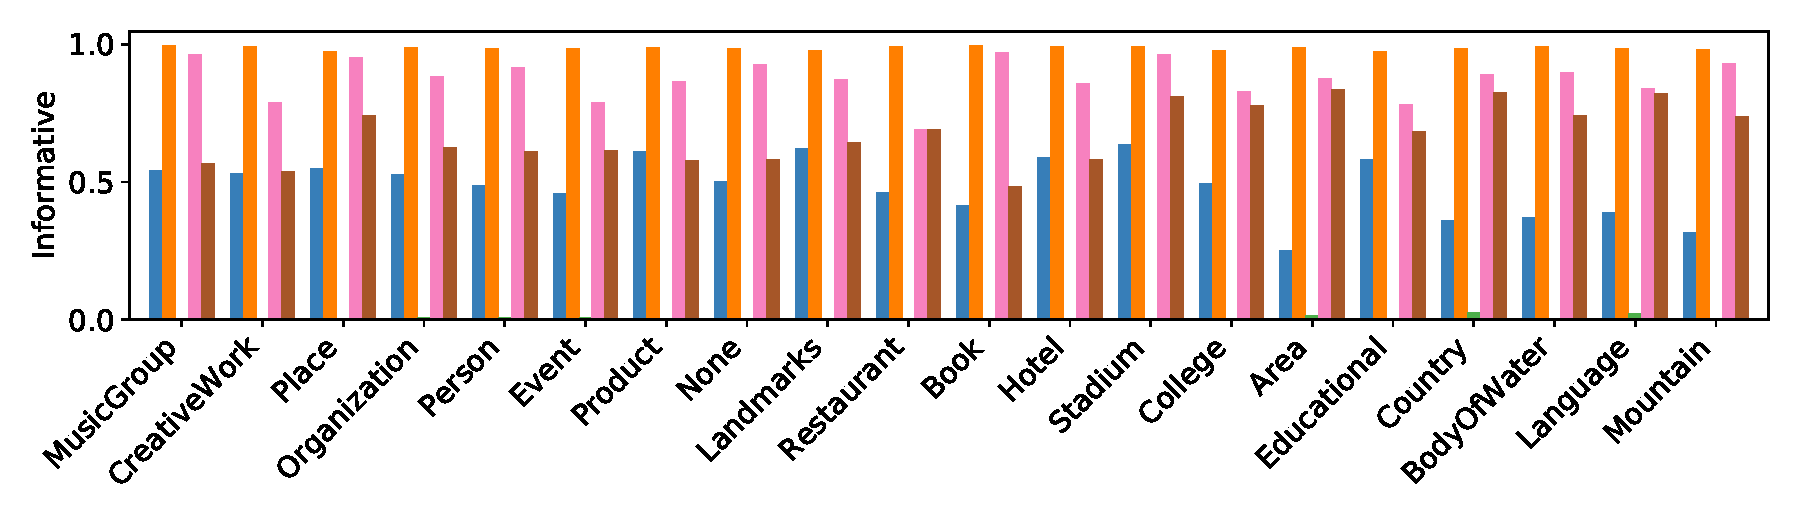
\includegraphics[width=5.5in]{submissions/Jing2024/figures/experiments/relation_analysis/informative_by_head_type.pdf}
 \label{fig:informative_by_head_type}
}\\

\includegraphics[width=5.5in]{submissions/Jing2024/figures/experiments/relation_analysis/legend.pdf}
\\\vspace{-6mm}
\subfloat[\textit{Informativeness} vs Tail entity type]{
 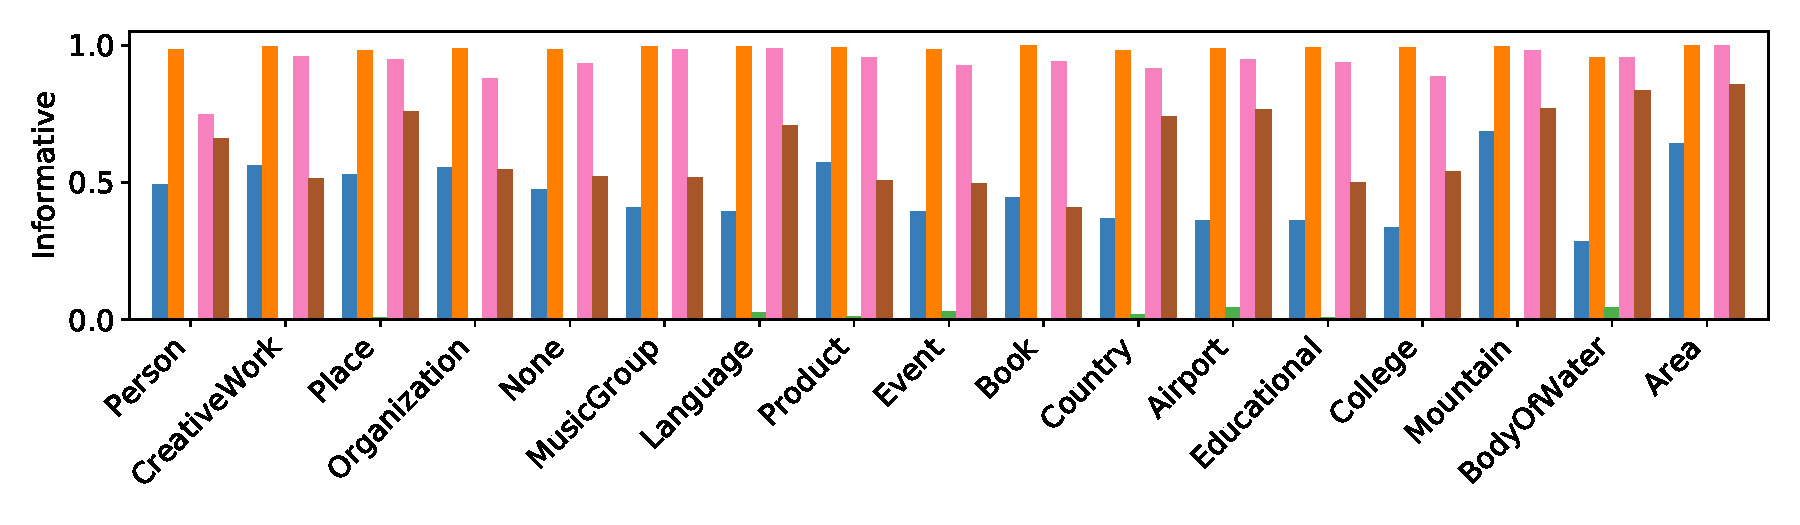
\includegraphics[width=5.5in]{submissions/Jing2024/figures/experiments/relation_analysis/informative_by_tail_type.pdf}
 \label{fig:informative_by_tail_type}
}
\caption{The LLM's \textit{informativeness} with respect to head entity types and tail entity types}
\label{fig:informativeness_by_type}
\end{figure}


